\chapter{Thesis \& methodology}
\label{chap:methodo}
\resetallacronyms

\begin{shaded}
  This chapter states first that multistage oil-free variable-speed
  domestic heat pumps powered by twin-stage radial compressors are
  feasible and demonstrate a significant potential. Then, it offers a
  methodology to validate this statement.
\end{shaded}

\Cref{chap:intro} states that better domestic heating systems are
needed and that heat pumps are one of the best candidates for this
improvement. \Cref{chap:sota} demonstrates that multistage oil-free
variable-speed technologies show promising perspectives in the heat
pumps application fields. Moreover, a twin-stage oil-free radial
compressor dedicated to heat pumps applications is being developed
based on a previous thesis work \citep{schiffmann-2008a}. The
integration of the single-stage unit in a refrigerant circuit has
shown promising results \citep[p.\,221]{schiffmann-2008a}, even if
that refrigerant circuit was not a single stage heat pump circuit
yet. Consequently, the purpose of this doctoral thesis is to push
further the integration and experiments performed by
\citet{schiffmann-2008a} with a single-stage compressor unit, using
now a twin-stage compressor unit and thus to demonstrate that
\textbf{multistage oil-free variable-speed domestic heat pumps powered
  by twin-stage radial compressors are feasible and demonstrate a
  significant potential}. This chapter describes the methodology used
in this work to achieve the demonstration of those two points. The
approach chosen is experimental and uses energy modeling to analyze
the behavior of the prototypes from laboratory measurements. Two
prototypes are being used for this demonstration: a pre-industrial
\AWP{} (further described in \cref{chap:awp}) and a more academic
\BWP{} (further described in \cref{chap:bwp}).

\section{Demonstration of feasibility}
\label{sec:feasability-demo}

The feasibility of the heating devices mentioned in the previous
section is demonstrated experimentally directly. Two prototypes, the
\AWP{} and the \BWP{}, have been designed, assembled, then
characterized with one \OP{}, or more (6 \OP{} have been tested for
the \AWP{}, including the A-7/W35 \OP{}, and 1 \OP{} for the
\BWP{}). The issues encountered and paths of improvement for those
prototypes are discussed in \cref{chap:awp,chap:bwp}.

\section{Demonstration of potential}
\label{sec:potential-demo}

In order to quantify the performance of the heat pump prototypes and
their components, measurements of physical values are needed at many
locations in the circuits of the prototypes. The measured physical
values include, from a thermodynamic point of view, pressure,
temperature, and mass flow rate measurements. However, many of those
locations do not easily allow to measure those physical values: Some
locations are very difficult to instrument, some measurements would
influence the behavior of the prototypes and/or decrease their
performance, some flow rates are very small and located in
inaccessible locations. For instance, the internal heat energy fluxes
and gas flow rates inside the compressor unit are complex and hard to
measure, especially in locations such as gas bearings and labyrinth
seals. An other example is the flow rate measurements in the \AWP{}
where compactness matters; it has been decided to leave the main flow
rates unmeasured in that prototype in order to match the compactness
criteria (report to \cref{sec:awp-description} for more details about
this choice). In order to compensate for those missing measurements, a
modeling approach is proposed. The proposed model propagates the
measured physical values and their uncertainties, through mass and
energy balance equations, to inaccessible locations. Those enhanced
results are used to characterize the performance of the prototypes and
spot the elements to improve, thus demonstrating the potential of the
technology. Historically, the \BWP{} has been designed and built
first, in 2009. It has been tested in 2010 unsuccessfully with
defectuous twin-stage compression units, and consequently gave
inexploitable \OP{} at the time, but contributed to gain experience
with the technology. The \BWP{} was more an acedemic experimental
setup than an industrial prototype, with lots of instrumentation and
modularity. Details about the \BWP{} are given in \cpref{chap:bwp},
and \cpref{chap:bwp-components}. The \AWP{}, designed and built in
2011 and 2012, has been tested while the testing of the \BWP{} had
been put on hold, and allowed to reach stable \OP{}, detailed in
\cref{chap:awp}. The \AWP{} is also a step into more integration of
the compression unit inside the heat pump circuits and was equipped
with an economizer coupled with the compression unit directly. The
details of this coupling is shown in \cpref{sec:awp-eco}. Details
about the \AWP{} are given in \cpref{chap:awp}, and
\cpref{chap:awp-components}. Building onto the experience gained with
the \AWP{}, the original \BWP{} has been modified, mainly to be able
to use the last generation of compression unit at the time, and in
order to test a new bypass system, likely to solve the issues observed
with the \AWP{}. The \AWP{} was more an industrial prototype than an
academic experimental setup and took advantage of the ideas and
thinking process which led to the design of the \BWP{}, and to some
extents, from the experience of the failed experiments performed on
the \BWP{} with the defectuous compression units. The modified \BWP{}
is presented in \cref{chap:bwp} and has been tested in 2013. The
experience gained with the two first prototypes suggests further
integration and ideas for the next prototypes. Those concepts and
proposals are exposed in \cpref{chap:cp-intg}.

\section{Limits of the demonstration}
\label{sec:methodo-limits}

The methodology proposed allows the demonstration of the feasibility
of twin-stage oil-free variable-speed domestic heat pumps and the
potential of this technology for heat pumps applications. Autonomous
control and switching between modes such as defrosting-mode,
heating-mode, cooling-mode and start \& stop procedures are only
evoked in the form of remarks and comments and need further
developments and analysis, as they imply more dynamic tests of the
prototypes, which have not been performed so far. They are consequently
out of the scope of this thesis work. However, the remarks and
comments are inspired by the observations made during the experiments
and are summarized in \cref{chap:cp-intg}.


\section{Methodology}
\label{sec:methodology}

\subsection{Design and assembly of heat pump prototypes}
\label{sec:methodo-design}

The design and assembly of the heat pump prototypes follow traditional
heat pumps systems design rules, as detailed in various references
\citep{rapin-desmons-2011a,Brown-1997a,Smith-Zappe-2004a,ASHRAE-HVACeq-2008a-HX,ASHRAE-HVACeq-2008a-Valves},
but add also some specific rules that are related to oil-free
technologies. Some of these specific rules add constraints, some give
more flexibility. Those additional design rules, often learned while
developing the successive versions of the prototypes of the heat pumps
presented in this work, are presented in \cref{chap:cp-intg}. Only the
last versions of the prototypes, which have been used for the tests
and to generate the results, are presented in details in
\cref{chap:awp,chap:bwp} and their appendix.

\subsection{Test of the heat pump prototypes}
\label{sec:methodo-tests}

The prototypes have been tested many times with different versions of
the compression units. Most of those units have been destroyed before
any interesting \OP{} could be reached, unfortunately. The tests
presented in this work have been performed using two of the first
functional twin-stage compression units available during the whole
thesis time\footnote{The compression unit mounted in the \BWP{} was
  the unit named \textit{cp101} and compression unit mounted in the
  \AWP{} was the unit named \textit{cp105}. Both were issued from the
  design family of the prototypes of the compression unit named
  \textit{evo4}. Both have been destroyed during the tests at
  EPFL. The unit \textit{cp105} has been tested in May 2012. The unit
  \textit{cp101} has been used in the industrial partners laboratories
  in 2011 and 2012, for heatpump tests, and has been tested at EPFL
  only after, in 2013.}. The units used in \BWP{} and \AWP{} have been
destroyed during the tests. The development of the compression units
has been carried on, and fully functional twin-stage compression
units, with a advanced designs, have been finalized between 2013 and
2015, and are now available. Their design have evolved and they are
now incompatible with the prototypes of the heat pumps developed
during this thesis (mainly because the location of their inlets and
outlets have been modified). The prototypes of the heat pumps need to
be modified to integrate the new cores. Further details about the
compression units and their compatibility with the prototypes of the
heat pumps can be found in \cref{chap:cp-intg}. The \OP{} presented in
this thesis work are the \OP{} that could be reached with the
prototypes before the compression unit was destroyed, for the case of
the \BWP{}, or before the \AWP{} prototype was shipped to the
industrial partner. Tests were carried out starting with a steady
state system at a given uniform temperature (at the climate chamber
temperature for the \AWP{} and at the atmospheric temperature for the
\BWP{}). The difference between the sources temperatures being slowly
increased gradually during the tests. Every \OP{} presented in this
work is stable conditions recorded during those slow increase
procedures: when a stable point was found, it was recorded, keeping
the system in that stable state for at least 10 minutes. Each stable
\OP{} presented is in fact an average of the measurements performed
during the more stable 3-minute period during the stable period of at
least 10 minutes. The data acquisition rate was at minimum of 1
measurement per second, which gives an interesting level of accuracy
of the \OP{} measurements (see \cref{chap:uncert} for details about
uncertainties and uncertainty calculations).

\subsection{Modeling of those heat pump prototypes}
\label{sec:methodo-models}

\begin{figure}
  \centering
  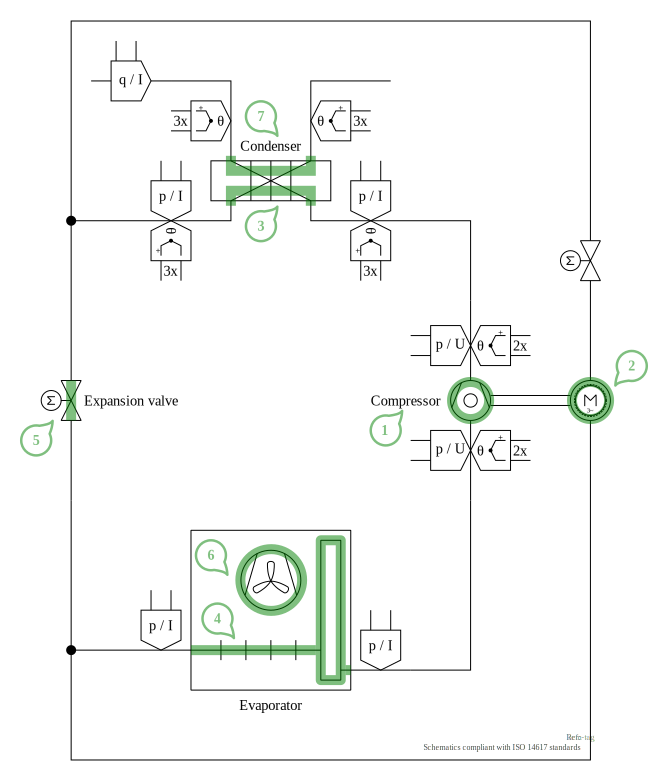
\includegraphics[width=0.9\textwidth]{simple-example-layout}
  \begin{tabular}[h]{cc}
    \includegraphics[width=0.45\textwidth]{simple-example-model} &
    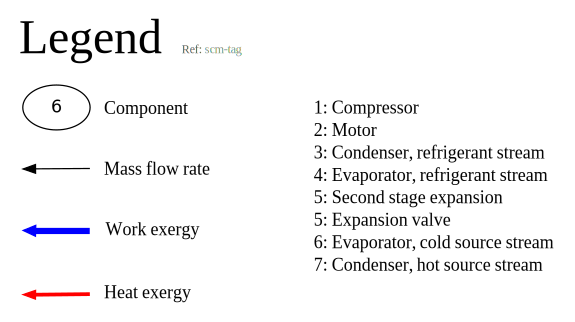
\includegraphics[width=0.45\textwidth]{simple-example-model-legend}\\
  \end{tabular}
  \caption[Example case -- Layout \& model]{Example case - Layout \&
    model of a single-stage heat pump. Symbols are compliant with the
    \cite{ISO14617}\,14617 standards.}
  \label{fig:simple-example-layout+model}
\end{figure}

The modeling methodology follows the steps detailed below:

\begin{description}
\item [Draw a layout of the installation and the frontier of the
  analysis]where \textbf{all} the flow rates and possible entities
  appear. All the existing flow rates need to be visible on the
  layout.
\item[Separate the layout in components.] A component is a network, as
  intended by \citet[p.\,24--25]{Borel-Favrat-2010a}, and corresponds
  to an element where flows enter and leave, partially (if there are
  accumulation) or totally, and that can exchange energy with normal
  components, or special components like the atmosphere or the
  environment of the device. The special components have no flow and
  are infinite reservoir at a given temperature. They can exchange
  energy with normal components or be the source or the receiver of
  flows. With this paradigm, a component does not necessarily
  correspond to a physical element or to a part of the system that can
  be isolated from the rest. For instance, a heat exchanger, in this
  paradigm, is made of two components which exchange heat energy. In
  the next chapters, the compression unit will be modeled as many
  components exchanging mass or energy (details about this modeling of
  the compression unit are given in \cref{chap:awp} \&
  \cref{chap:bwp}). This thesis work uses steady-state models. In
  steady state conditions, mass and energy balances are equal to zero
  for every components, as for the whole system delimited by a
  frontier. There is no mass change of the components. The components
  are assigned with a number. The modeling approach presented here
  could also be used to generate quasi-static models or dynamic
  models, if enough data is available.
\item[Transform the layout view into the model view.] Each component
  exchanges energy or mass with other components. The representation
  of the model using the GraphViz modeling paradigm from
  \citet{Gansner-North-2000a}, typically dedicated to sofware
  engineering modeling, is unusual in the thermodynamic modeling field
  and is a representation analogy proposed by the author of this
  thesis work. In the opposite, the modeling itself, using mass and
  energy balances is a common modeling approach in the thermodynamic
  field. Each type of energy is represented with a bold and colored
  arrow, and the mass flow rates are represented with thin black
  arrows. The convention is that positive energy or mass flow rates
  enter the components. Negative flows leave the components. This
  means that a negative value results in a flow moving against the
  arrow. The notation indicates the direction of the arrow with
  subscripts using the numbers or the components, separated by an
  arrow.
\item[Determine the equations.] Each components gives two equations: a
  mass flow rates balance equation, as shown in
  \cref{eq:mass-balances-eq-general}, and an energy rates balance
  equation, as shown in \cref{eq:energy-balances-eq-general}. By
  convention, each transformation energy rate\footnotep{See
    \cpref{sec:methodo-defs}, for a definition of the transformation
    energy rate.} is included in the equation using the outlet
  specific enthalpy\footnotep{See \cpref{sec:methodo-defs}, for a
    definition of the specific enthalpy.} of the component being the
  source of this flow rate. The whole device, at its frontier, also
  provides a mass flow rates balance equation and an energy rates
  balance equation. In the case of dynamic modeling, the mass and
  energy balance equations are not equal to zero. A steady-state
  approach has been favored in this thesis work because the data
  collected during the experiments were not enough to solve equations
  not equal to zero\footnotep{Fitting a dynamic model of the
    prototypes would have required to know the variation of mass of
    the components. Most of the components mass variation can be
    neglected, but the variation of mass of the condenser, the
    evaporator, and the economizer need to be measured (or,
    alternatively, the mass flow rates entering and leaving those
    components can be measured, but this is technically far more
    difficult and inconvenient). Those measurements were planned to be
    made in the BWP, but most of the experiments have been performed
    on the AWP. The BWP has only given a single OP and the load cells
    were not calibrated at the time, as this is a procedure which was
    planned for the next experiments. For more details, see
    \cpref{chap:awp}, and \cpref{chap:bwp}.}.

\begin{equation}
  \label{eq:mass-balances-eq-general}
  \sum^n_{i=1} \dot{M}_{x_i \rightarrow y_i} = 0
  \tagaddtextone{$\left[\si{\watt}\right]$}
\end{equation}

\begin{equation}
  \label{eq:energy-balances-eq-general}
  \sum^m_{i=1} \dot{M}_{a_i \rightarrow b_i} \cdot h_{out\,a_i} +
  \sum^n_{j=1}\dot{Y}_{c_j \rightarrow d_j} +
  \sum^p_{k=1}\dot{E}_{e_k \rightarrow f_k} = 0
  \tagaddtextone{$\left[\si{\watt}\right]$}
\end{equation}

\item[Solve the system of equations.] Mass flow rates balance
  equations have the priority. They are solved first, if
  possible. When no more equations can be solved, a fitting parameter
  is added with the introduction of a new relation bounding 2
  variables together. For instance, this can be introduced for a flow
  which is divided in two. The proportion of the entering flow leaving
  in one of the leaving flows is characterized here with a splitting
  parameter. When all the mass flow rates are determined, the energy
  balance equations are written with the same method.

\item[Implement the model.] As soon as every variable can be
  expressed, the model is implemented in a modeling software (here,
  the MATLAB from MathWorks) and the set of equations is solved with a
  solver. The solver tries to fit the parameter that were added to
  express every variable as an expression in order to get the lowest
  objective function value. If no fit parameter was added, the level
  of information of the system is sufficient and the set of equations
  should close, within the limits of the measurement uncertainty
  ranges. A set of equations is considered closed, in steady state
  conditions, if every energy and mass balance of every component and
  the balances at the frontier of the system are equal to zero. If fit
  parameters were added, the set of equations is now solvable but is
  not closed. Consequently, a fitting of those parameters is necessary
  to close the system. This step is performed using a minimization of
  an objective function under constraints, using a standard
  optimization algorithm. In this work, the MATLAB
  \textit{fmincon}\,\citep{fmincon2014a} function has been used with
  an interior point algorithm, which was the best suited to solve this
  problem with this function \citep{fmincon2014a-interiorpoint}. The
  variables of this algorithm are the fit parameters. Constraints on
  the variables are necessary to bound the fit parameters and to
  ensure that realistic conditions only are explored by the
  algorithm. For instance, if a flow is divided into three flows using
  two fit parameters, the sum of those two parameters can not be
  greater than one. The starting point of the minimization algorithm
  is determined randomly. The first valid starting point found
  randomly is selected as the optimization starting point. Indeed, the
  fluid properties at each location in the cycles are determined using
  the \REFPROP{} \citep{REFPROP90} but the latter can only compute
  properties within given inputs range. When the number of fit
  parameters starts to be quite high, as this is the case with the
  \AWP{} model, it is common that a randomly chosen starting point is
  not defined which implies that the minimization algorithm does not
  initialize. The objective function minimized by the optimizer is the
  sum of two aggregates of indicators. The first one has an order of
  magnitude above $\num{1e0}$ and is the sum of an array. This array
  contains statements penalizing unrealistic conditions in the system,
  such as an outlet stream enthalpy lower than its inlet stream
  enthalpy, in a compressor. If an unrealistic condition is observed,
  the objective function is penalized using the difference between the
  realistic condition that should be and its current unrealistic
  state. In other word, the more the condition is unrealistic the
  bigger is the penalization. This first term, as soon as the system
  is realistic, is equal to zero. If this term is not equal to zero,
  the solution found by the optimizer is not considered, an other
  starting point is chosen, and the optimizer is run again. The second
  term of the sum is of an order of magnitude below $\num{1e0}$ and
  corresponds to the sum of the energy balances on every component and
  on frontier of the system. It is equal to zero when all the balances
  are equal to zero. Typically, this term is never exactly equal to
  zero due to the fact that a model never fully represents the reality
  and due to uncertainties and measurement errors. The optimization
  problem has been run for every experimental points more that a
  hundred times in order to provide more confidence in the presented
  results. For the points presented in this work the sum of those
  balances is always below 100W.
\item[Analyze the results] As soon as the parameters of the system
  have been fitted, an analysis of the system can be performed.
\end{description}

In order to better understand this modeling approach, a simple example
dedicated to illustrate the methodology is offered here. The chosen
example is a single stage heat pump using part of the liquid
refrigerant leaving the condenser to cool down the motor of the
compressor. The partly evaporated flow is then collected at the
evaporator inlet. The layout of this heat pump is presented in
\cref{fig:simple-example-layout+model}. Using the modeling approach
proposed above, the example system is modeled using 7 components. This
model is described in \cref{fig:simple-example-layout+model}. The
components are represented on the layout with green markers and are
listed in the legend provided with the model.

Unfortunately, the designer of this example experimental setup, for
unknown reasons, could not instrument the heat pump with enough
sensors. Each component of the system can not be characterized and
only some physical values are available. The measurement points are
represented on the layout in \cref{fig:simple-example-layout+model}. A
\gls{glos:bold} is a value physically measured in the experiment. An
\gls{glos:underline} is guessed directly by the optimizer, and a
\gls{glos:normal-font} is computed with the model\footnotep{See the
  glossary at the beginning of the thesis for details about the
  signification of those 3 types of values.}. The uncertainties are
being propagated through the model\footnotep{See \cpref{chap:uncert}
  for more details about uncertainties computation and
  propagation.}. For the example case, the values are presented in
\cref{tab:simple-example-PThs,tab:simple-example-dotEQ}.

\begin{table}[ht!]
  \footnotesize
  \begin{center}
    \begin{tabular}{cccccc}
\toprule
Component & Location & P / \si{\bar} & T / \si{\degreeCelsius} & h / \si{\kilo\joule\per\kilo\gram} & s / \si{\kilo\joule\per\kilo\gram\per\kelvin}\\
\midrule
\multirow{2}{*}{1} & inlet & \textbf{3.50 +/- 0.05} & \textbf{8.53 +/- 0.15} & 404.72 +/- 0.27 & 1.7359 +/- 0.0020\\
& outlet & \textbf{9.12 +/- 0.05} & \textbf{86.01 +/- 0.27} & 469.78 +/- 0.35 & 1.8689 +/- 0.0014\\
\midrule
\multirow{2}{*}{2} & inlet & \textbf{4.30 +/- 0.05} & 11.10 +/- 0.35 & 243.18 +/- 0.22 & 1.1526 +/- 0.0014\\
& outlet & \textbf{3.70 +/- 0.05} & 6.64 +/- 0.39 & 382.00 +/- 0.22 & 1.6507 +/- 0.0000\\
\midrule
\multirow{2}{*}{3} & inlet & \textbf{9.12 +/- 0.05} & \textbf{86.01 +/- 0.15} & 469.78 +/- 0.22 & 1.8689 +/- 0.0010\\
& outlet & \textbf{8.52 +/- 0.05} & \textbf{31.01 +/- 0.15} & 243.18 +/- 0.22 & 1.1481 +/- 0.0007\\
\midrule
\multirow{2}{*}{4} & inlet & \textbf{3.70 +/- 0.05} & 6.64 +/- 0.39 & 245.81 +/- 17.47 & 1.1639 +/- 0.0015\\
& outlet & \textbf{3.50 +/- 0.05} & 8.53 +/- 0.44 & 404.72 +/- 0.27 & 1.7359 +/- 0.0020\\
\midrule
\multirow{2}{*}{5} & inlet & 8.52 +/- 0.05 & 31.01 +/- 0.15 & 243.18 +/- 0.22 & 1.1481 +/- 0.0007\\
& outlet & 3.70 +/- 0.05 & 6.64 +/- 0.39 & 243.18 +/- 0.22 & 1.1545 +/- 0.0015\\
\midrule
\multirow{2}{*}{6} & inlet & \textbf{1.00 +/- 0.05} & \textbf{10.00 +/- 0.15} & 407.21 +/- 0.16 & 3.8055 +/- 0.0149\\
& outlet & \textbf{1.00 +/- 0.05} & \textbf{7.00 +/- 0.15} & 404.20 +/- 0.16 & 3.7948 +/- 0.0149\\
\midrule
\multirow{2}{*}{7} & inlet & \textbf{2.00 +/- 0.05} & \textbf{30.00 +/- 0.15} & 125.91 +/- 0.63 & 0.4367 +/- 0.0021\\
& outlet & \textbf{1.70 +/- 0.05} & \textbf{35.00 +/- 0.15} & 146.78 +/- 0.63 & 0.5051 +/- 0.0020\\
\bottomrule
\end{tabular}

  \end{center}
  \caption{Example case -- Thermodynamic points of the heat pump cycle}
  \label{tab:simple-example-PThs}
\end{table}

In order to compensate for the missing measurements, the heat pump
system is modeled with the proposed approach. The known mass flows and
energy fluxes are identified and used to write the set of equations in
a solvable order. The set of equations is detailed for this example
case in \cpref{chap:simple-model-equations-set}. The set of equations
is solved, starting with mass flow rates balance equations. When the
resolution is stopped by uncharacterized flows, a fit parameter is
added. For instance, in the example case, the refrigerant flow coming
from the compressor (component \#1) is divided after the condenser
circuit (component \#3) into two streams. The splitting of this flow
between those two streams is unknown. Consequently, a split factor is
added and will later be fitted in order to close the set of equations
(in the example case, the fit parameter $f_{01}$ is introduced with
\cref{eq:simple-model-equations-set-factor01}). As soon as every mass
flow is characterized, eventually using fit parameters, the same
procedure is applied to energy fluxes, starting with known fluxes, and
using equations similar to \cref{eq:energy-balances-eq-general}. When
the resolution is stopped by uncharacterized fluxes, a fit parameter
is also added. At the end of this process, the whole system is
characterized using the thermodynamic conditions at the measurement
points and the measured flows and fluxes. In the example case
considered in this chapter, this model allows to determine the values
presented in
\crefrange{tab:simple-example-PThs}{tab:simple-example-dotEQ}, to draw
diagrams such as the ones presented
\cref{fig:simple-example-diagrams}, and to determine performance
indicators, such as the \COP{}, which is here of 3.35, or such as the
motor efficiency, which is equal to ~\SI{96.11}{\%}
here\footnotep{Those performance indicators are defined in section
  \cref{sec:methodo-analysis}.}.

\begin{table}[htb]
    \footnotesize
    \begin{center}
    \begin{tabular}{llllll}
\toprule
Name & Value / \si{\gram\per\second} & Name & Value / \si{\gram\per\second} & Name & Value / \si{\gram\per\second} \\
\midrule
$\dot{M}_{1 \rightarrow 3}$ & 32.2336 +/- 1.65904 & $\dot{M}_{2 \rightarrow 4}$ & 0.611456 +/- 0.0314711 & $\dot{M}_{3 \rightarrow 2}$ & 0.611456 +/- 0.0314711 \\
$\dot{M}_{3 \rightarrow 5}$ & 31.6221 +/- 1.62757 & $\dot{M}_{4 \rightarrow 1}$ & 32.2336 +/- 1.62787 & $\dot{M}_{5 \rightarrow 4}$ & 31.6221 +/- 1.62757 \\
$\dot{M}_{6 \rightarrow en}$ & 1697.52 +/- 180.24 & $\dot{M}_{7 \rightarrow ho}$ & \textbf{350 +/- 10} & $\dot{M}_{en \rightarrow 6}$ & 1697.52 +/- 180.24 \\
$\dot{M}_{ho \rightarrow 7}$ & 350 +/- 10 \\
\bottomrule
\end{tabular}

  \end{center}
  \caption{Example case -- Mass flow rates between the components}
  \label{tab:simple-example-dotM}
\end{table}

\begin{table}[htb]
    \footnotesize
    \begin{center}
    \begin{tabular}{llll}
\toprule
Name & Value / $W$ & Name & Value / $W$ \\
\midrule
$\dot{E}_{2 \rightarrow 1}$ & 2097.11 +/- 108.52 & $\dot{E}_{el \rightarrow 2}$ & \textbf{2182.00 +/- 1.00} \\
$\dot{Y}_{3 \rightarrow 7}$ & 7304.18 +/- 375.81 & $\dot{Y}_{6 \rightarrow 4}$ & 5122.18 +/- 375.81 \\
\bottomrule
\end{tabular}

  \end{center}
  \caption{Example case -- Energy flows between the components}
  \label{tab:simple-example-dotEQ}
\end{table}

\begin{figure}[htb]
  \centering
  \subfloat[Refrigeration diagram]
  {\label{fig:simple-example-Ph}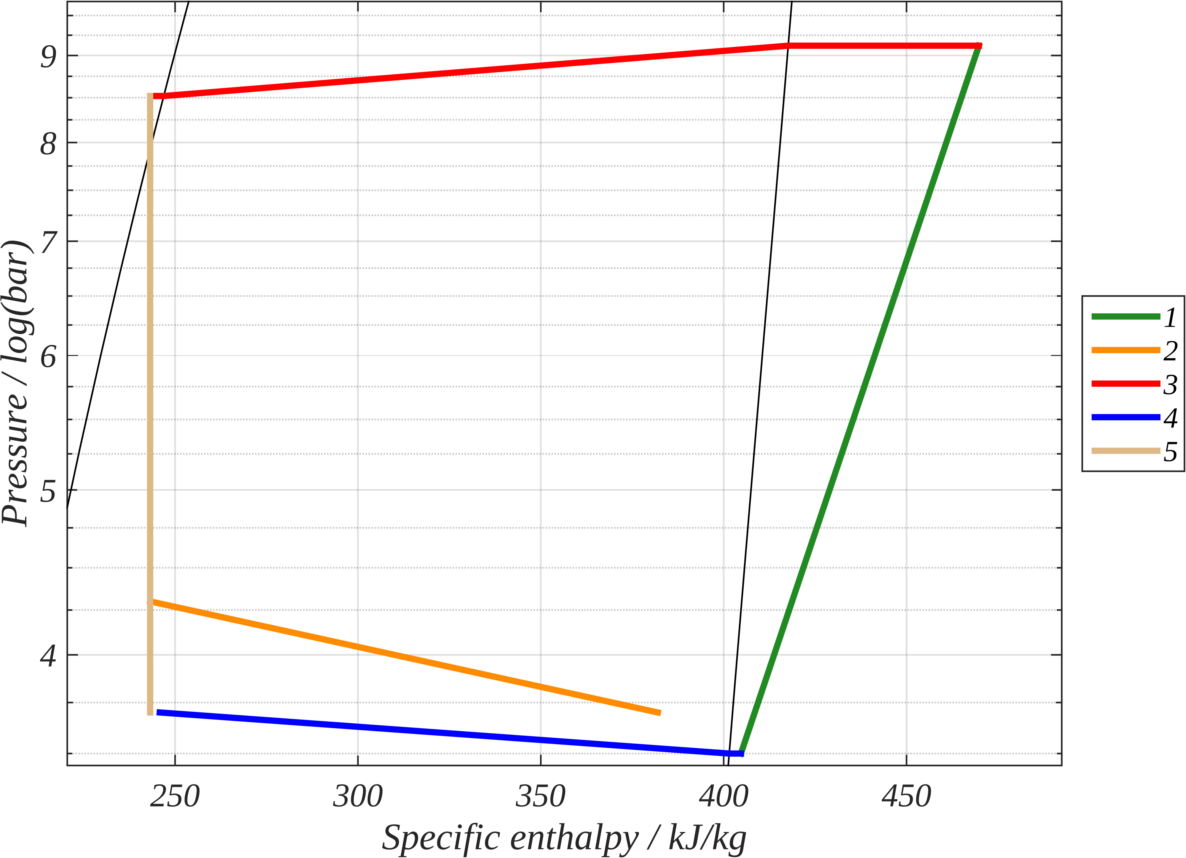
\includegraphics[width=0.45\textwidth]{simple-example-Ph}}
  \hspace{1em}
  \subfloat[Entropic diagram]
  {\label{fig:simple-example-Ts}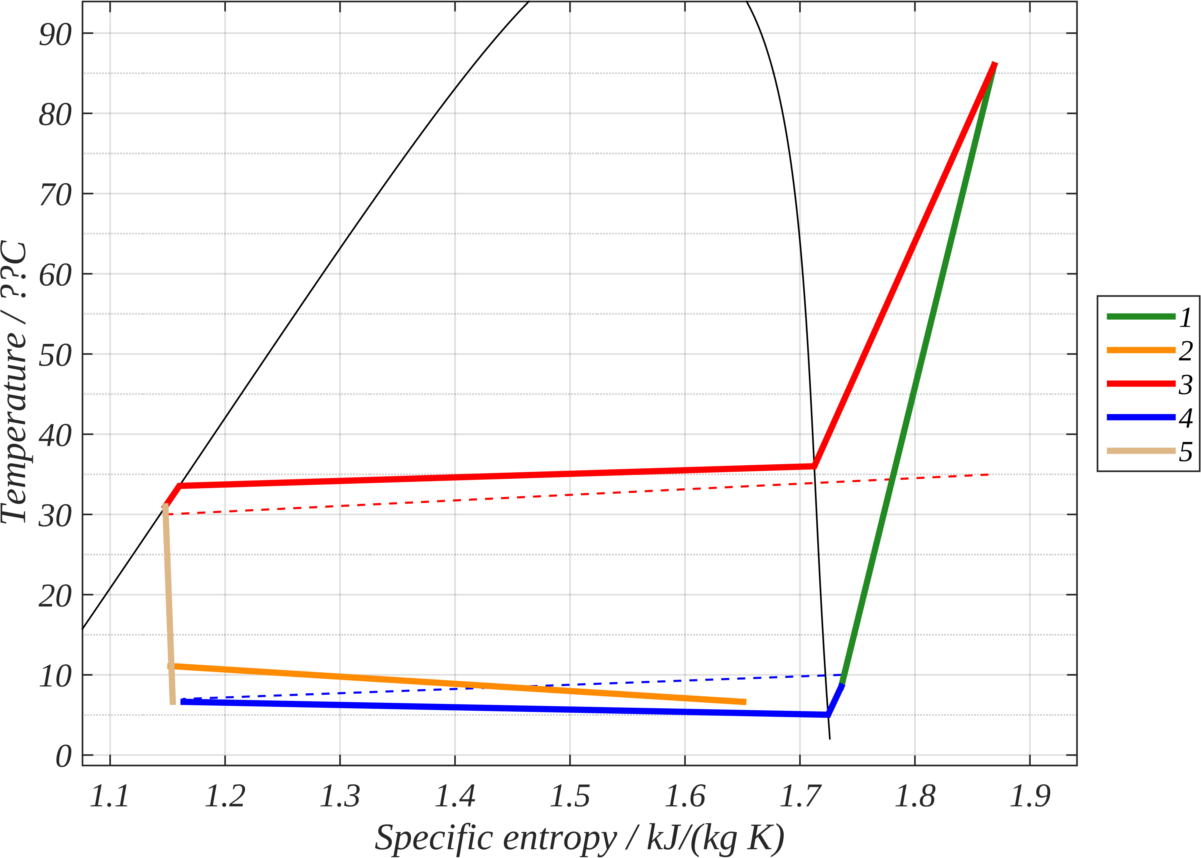
\includegraphics[width=0.45\textwidth]{simple-example-Ts}}
  \caption[Example case -- Thermodynamic diagrams]{Example case --
    Thermodynamic diagrams. The legend of the numbered lines is
    available on \cref{fig:simple-example-layout+model}. Dashed lines
    represent the sources.}
  \label{fig:simple-example-diagrams}
\end{figure}

\subsection{Analysis of the experimental results}
\label{sec:methodo-analysis}

The experimental results are analyzed using diagrams, and performance
indicators, which are defined below.

\subsubsection{Definitions}
\label{sec:methodo-defs}

\paragraph{Pressure ratio ($\Pi$):}

The pressure ratio is the ratio of the absolute pressure at the
compressor outlet to the absolute pressure at the compressor
inlet. Consequently, the first stage pressure ratio is the ratio of
the absolute pressure at the first stage compressor outlet
$P_{1,\,out}$ to the absolute pressure at the first-stage compressor
inlet $P_{1,\,in}$. The second stage pressure ratio is the ratio of
the absolute pressure at the second stage compressor outlet
$P_{2,\,out}$ to the absolute pressure at the second stage compressor
inlet $P_{2,\,in}$. Those two ratios are defined in \cref{eq:PR}.

\begin{subequations}
  \label{eq:PR}
  \begin{align}
  \Pi_1 = \dfrac{P_{1,\,out}}{P_{1,\,in}}
  \tagaddtexttwo{$\left[-\right]$} \\
  \Pi_2 = \dfrac{P_{2,\,out}}{P_{2,\,in}}
  \tagaddtexttwo{$\left[-\right]$}
  \end{align}
\end{subequations}

% \paragraph{Mass flow rate ($\dot{M}$)}


\paragraph{Specific enthalpy ($h$):}

The specific enthalpy is a state function resulting of the combination
of the specific internal energy $u$, the specific volume $v$, and the
pressure $P$ state functions \citep[p.\,19]{Borel-Favrat-2010a}. It is
computed as described in \cref{eq:h}. The specific enthalpy is used in
the energy rate calculations.

\begin{equation}
  \label{eq:h}
  h = u + vP
  \tagaddtextone{$\left[\si{\joule\per\kilo\gram}\right]$}
\end{equation}

\paragraph{Specific entropy ($s$):}
The specific entropy is a state function which may vary as a result of
transfers across the system boundary or because of internal processes
of the system which result in entropy creation
\citep[p.\,37]{Borel-Favrat-2010a}. The specific entropy unit is
\si{\joule\per\kilo\gram\per\kelvin}. It is used in various
thermodynamic calculations, and especially in exergy calculation, via
the coenthalpy.


\paragraph{Specific coenthalpy ($k$):}
The specific coenthalpy is a state function defined from the specific
enthalpy $h$, the environment temperature $T_a$ and the specific
entropy $s$, as described in \cref{eq:k}
\citep[p.\,410]{Borel-Favrat-2010a}. The specific coenthalpy is used
in the exergy rate calculations. The environment temperature $T_a$ is
the temperature of the air at the inlet of the evaporator, for the
\AWP{}, and of the room temperature for the \BWP{}.

\begin{equation}
  \label{eq:k}
  k = h + T_a\,s
  \tagaddtextone{$\left[\si{\joule\per\kilo\gram}\right]$}
\end{equation}

\paragraph{Transformation energy rate ($\dot{Y}$):}

\citet[p.\,24]{Borel-Favrat-2010a} define the transformation energy
rate as defined in \cref{eq:dotY}. Normally, the transformation energy
rate is decreased by the derivative of the quantity $U + P_aV$,
relative to time, $U$ being the internal energy, $P_a$ being the
pressure of the environment, and $V$ being the volume. The derivative
of this quantity being equal to zero or being negligible for the
system studied here, it is not mentioned in \cref{eq:dotY}.

\begin{equation}
  \label{eq:dotY}
  \dot{Y}^{+} = \sum_{j} h_j \, \dot{M}_j^{+}
  \tagaddtextone{$\left[\si{\watt}\right]$}
\end{equation}

\paragraph{Transformation exergy rate ($\dot{E}_{y}$):}

Based on the transformation energy rate, the transformation exergy
rate is defined as described in \cref{eq:dotEy}
\citep[p.\,410]{Borel-Favrat-2010a}. Normally, the transformation
exergy rate is decreased by the derivative of coenergy $J$ relative to
time. The coenergy is defined as $J = U + P_aV-T_aS$ with $U$, the
internal energy, $P_a$ the environment pressure, $T_a$, the
environment temperature, $V$, the volume, and $S$, the entropy. The
derivative of this quantity being here equal to zero or being
negligible for the system being studied here, it is not mentioned in
\cref{eq:dotEy}.

\begin{equation}
  \label{eq:dotEy}
  \dot{E}_{y}^{+} = \sum_{j} k_j \, \dot{M}_j^{+}
  \tagaddtextone{$\left[\si{\watt}\right]$}
\end{equation}

\subsubsection{Performance indicators}
\label{sec:methodo-indicators}

The components numbers which are used in the definitions are defined
in \cpref{fig:awp-layout-model-numbers} for the \AWP{} and in
\cpref{fig:bwp-maillefer-break-model} for the \BWP{}.

\paragraph{Heating effectiveness ($COP_h$):}

The heating effectiveness $\epsilon_h$, also called heating
Coefficient Of Performance ($COP_h$), is the ratio between heat power
$\dot{Q}^{-}_h$ supplied to the hot source and the consumed work power
$\dot{E}^{+}$. This definition can also be given in energy instead of
power, as defined by \citet[p.\,641]{Borel-Favrat-2010a}. It is
defined in \cref{eq:COPh}.

\begin{equation}
  \label{eq:COPh}
  \epsilon_h = COP_h = \dfrac{\dot{Y}^{-}_h}{\dot{E}^{+}} = \dfrac{\dot{Y}^{-}_{3 \rightarrow 15}}{\dot{E}^{+}_{el \rightarrow 14}}
  \tagaddtextone{$\left[-\right]$}
\end{equation}

\paragraph{Motor efficiency ($\eta_{mot}$):}

The motor efficiency is defined as the ratio between the work
transmitted to the shaft $\dot{E}^-_{\text{shaft}}$ and the electric
power consumed by the motor $\dot{E}^+_{\text{mot}}$. It is defined in
\cref{eq:eta_mot}.

\begin{equation}
  \label{eq:eta_mot}
  \eta_{mot} = \dfrac{\dot{E}^-_{\text{shaft}}}{\dot{E}^+_{\text{mot}}}
  \tagaddtextone{$\left[-\right]$}
\end{equation}

% \paragraph{Gas bearings effectiveness}

\paragraph{Isentropic efficiency ($\eta_s$):}

The isentropic efficiency of a compressor is defined as the ratio
between the isentropic work power of the compressor $\dot{E}_{cp,s}$,
which is the work power required by an adiabatic compressor without
dissipation performing an isentropic compression, and the actual work
$\dot{E}_{cp}$ required by the compressor. It is defined by
\cref{eq:eta_s_cp}.

\begin{equation}
  \label{eq:eta_s_cp}
  \eta_s = \dfrac{\dot{E}_{cp,s}}{\dot{E}_{cp}} = \dfrac{h_{out,s} - h_{in}}
  {h_{out} - h_{in}}
  \tagaddtextone{$\left[ - \right]$}
\end{equation}

The compressor inlet specific enthalpy $h_{in}$ is computed using the
inlet absolute pressure $P_{in}$ and temperature $T_{in}$. The
compressor isentropic outlet specific enthalpy $h_{out,s}$ is computed
using the outlet absolute pressure $P_{out}$ and the inlet specific
entropy $s_{in}$. The compressor outlet specific enthalpy $h_{out}$ is
computed using the inlet absolute pressure $P_{out}$ and temperature
$T_{out} > T_{out,s}$. The isentropic efficiency ranges between 0 and
1 (1 is the ideal unreachable case) and typical values range between
0.7 and 0.8 for nowadays compressors.

In the specific case of the non-adiabatic compression unit tested, we
can differentiate the external isentropic efficiency, and the
isentropic efficiency of the impeller only. The isentropic efficiency
of the impeller only is not accurately known, as the mass flow rates
and the inlets and outlets temperatures are deduced from the models
presented \cref{sec:awp-model,sec:bwp-model} and not measured
directly. They are defined with \cref{eq:eps_cp1_s,eq:eps_cp2_s}. The
external isentropic efficiencies include the leakage through the
labyrinth seal and the gas flux from the axial bearing to the inlet of
the first impeller. They are the isentropic efficiencies as measurable
from the outside of the unit, at its physical inlets/outlets and take
in account the different flows and energy transfers. Those isentropic
efficiencies are defined in \cref{eq:eps_cp1_s_ext,eq:eps_cp2_s_ext}
and are based on the definition offered by
\citet[p.\,201]{Borel-Favrat-2010a}.

\begin{equation}
  \label{eq:eps_cp1_s}
  \eta_{s,\,cp1} = \dfrac{\dotM{29}{1} \, h_{1,\,out,\,s} -
    \dotM{29}{1} \, h_{1,\,in} + \dot{Q}_{11 \rightarrow 1} -
    \dot{Q}_{1 \rightarrow 2}}{\dotM{29}{1} \, h_{1,\,out} - \dotM{29}{1} \,
    h_{1,\,in} + \dot{Q}_{11 \rightarrow 1} - \dot{Q}_{1 \rightarrow 2}}
  \tagaddtextone{$\left[-\right]$}
\end{equation}

\begin{equation}
  \label{eq:eps_cp1_s_ext}
  \eta_{s,\,cp1,\,ext} = \dfrac{\left( \dotM{10}{25} + \dotM{25}{27} +
      \dotM{25}{8} \right) \, h_{1,\,out,\,s} - \dotM{22}{29} \,
    h_{22,\,out} + \dot{Q}_{11 \rightarrow 1} - \dot{Q}_{1
      \rightarrow 2}}{\left( \dotM{10}{25} + \dotM{25}{27} +
      \dotM{25}{8} \right) \, h_{1,\,out} - \dotM{22}{29} \,
    h_{22,\,out} + \dot{Q}_{11 \rightarrow 1} - \dot{Q}_{1
      \rightarrow 2}}
  \tagaddtextone{$\left[-\right]$}
\end{equation}

\begin{equation}
  \label{eq:eps_cp2_s}
  \eta_{s,\,cp2} = \dfrac{\dotM{28}{2} \, h_{2,\,out,\,s} - \dotM{28}{2}
    h_{2,\,in} + \dot{Q}_{1 \rightarrow 2} - \dot{Q}_{2 \rightarrow
      10}}{\dotM{28}{2} \, h_{2,\,out} - \dotM{28}{2} h_{2,\,in} +
    \dot{Q}_{1 \rightarrow 2} - \dot{Q}_{2 \rightarrow 10}}
  \tagaddtextone{$\left[-\right]$}
\end{equation}

\begin{equation}
  \label{eq:eps_cp2_s_ext}
  \eta_{s,\,cp2,\,ext} = \dfrac{\left( \dotM{2}{10} + \dotM{2}{20}
    \right) \, h_{2,\,out,\,s} - \dotM{28}{2} \, h_{2,\,in} +
    \dot{Q}_{1 \rightarrow 2} - \dot{Q}_{2 \rightarrow 10}}{\left(
      \dotM{2}{10} + \dotM{2}{20} \right) \, h_{2,\,out} -
    \dotM{28}{2} \, h_{2,\,in} + \dot{Q}_{1 \rightarrow 2} -
    \dot{Q}_{2 \rightarrow 10}}
  \tagaddtexttwo{$\left[-\right]$}
\end{equation}

\paragraph{Exergy efficiencies ($\eta$):}

\citet[based on def.~p.\,2]{Favrat-Epelly-2008a} give a general
definition of the exergy linked to a transfer or a storage of energy
and define it as the potential of maximum work which could ideally be
obtained from each energy unit being transferred or stored (using
reversible processes exchanging heat only with the
atmosphere). \citet[p.\,406--448]{Borel-Favrat-2010a} give a detailed
explanation of the exergy approach applied to system analysis. They
develop the concept of exergy efficiency in general
\citep[p.\,447--448]{Borel-Favrat-2010a}, and apply it to the specific
case of a heat pump \citep[p.\,642]{Borel-Favrat-2010a}. Written using
exergy rates instead exergy, the exergy efficiency of a heat pump is
defined as the ratio between the supplied transformation exergy power
$\dot{E}^-_{yh}$ and the consumed electrical power
$\dot{E}^+_{el}$. This ratio is expressed mathematically in
\cref{eq:eta_heatpump}.

\begin{equation}
  \label{eq:eta_heatpump}
  \eta_{heatpump} = \dfrac{\dot{E}^-_{yh}}{\dot{E}^+_{el}} =
  \dfrac{\dotM{17}{15} \, \left( k_{15,\,out} - k_{15,\,in} \right)}
  {\dotE{el}{14}}
  \tagaddtexttwo{$\left[-\right]$}
\end{equation}


The exergy efficiency of the first compression stage is defined in \cref{eq:eta_cp1_awp} for the \AWP{}, and in \cref{eq:eta_cp1_bwp} for the \BWP{}.

\begin{subequations}
  \begin{align}
  \eta_{cp1} = \dfrac{\dotM{22}{29} \, \left( k_{25,\,out} - k_{29,\,in} \right)}{\dotE{11}{1} - \dotE{1}{2}}
  \tagaddtextthree{$\left[-\right]$} \label{eq:eta_cp1_awp} \\
  \eta_{cp1} = \dfrac{\dotM{19}{1} \, \left( k_{25,\,out} - k_{19,\,out} \right)}{\dotE{11}{1} - \dotE{1}{2}}
  \tagaddtextthree{$\left[-\right]$} \label{eq:eta_cp1_bwp}
  \end{align}
\end{subequations}

The exergy efficiency of the first compression stage is defined in
\cref{eq:eta_cp1_imp}.

\begin{equation}
  \label{eq:eta_cp1_imp}
  \eta_{cp1,\,imp} = \dfrac{\dotM{1}{25} \, \left( k_{1,\,out} - k_{1,\,in} \right)}{\dotE{11}{1} - \dotE{1}{2}}
  \tagaddtexttwo{$\left[-\right]$}
\end{equation}

The exergy efficiency of the second compression stage is defined in
\cref{eq:eta_cp2}.

\begin{equation}
  \label{eq:eta_cp2}
  \eta_{cp2} = \dfrac{\dotM{2}{20} \, \left( k_{2,\,out} - k_{2,\,in} \right)}{\dotE{1}{2}}
  \tagaddtexttwo{$\left[-\right]$}
\end{equation}

The exergy efficiency of the second stage impeller is defined in
\cref{eq:eta_cp2_imp_awp} for the \AWP{}, and in
\cref{eq:eta_cp2_imp_awp} for the \BWP{}.

\begin{subequations}
  \begin{align}
    \eta_{cp2,\,imp} = \dfrac{\dotM{28}{2} \, \left( k_{2,\,out} - k_{2,\,in} \right)}{\dotE{1}{2}}
    \tagaddtextthree{$\left[-\right]$} \label{eq:eta_cp2_imp_awp} \\
    \eta_{cp2,\,imp} = \dfrac{\dotM{27}{2} \, \left( k_{2,\,out} - k_{2,\,in} \right)}{\dotE{1}{2}}
    \tagaddtextthree{$\left[-\right]$} \label{eq:eta_cp2_imp_bwp}
  \end{align}
\end{subequations}

Component \#15 specific coenthalpies are determined using CoolProp
5.0.8 \citep{coolprop} Ethylen Glycol / Water mixture fluid
properties. Other fluid properties are computed using the \REFPROP{}
\citep{REFPROP90}. The exergy efficiency of the condenser is defined in \cref{eq:eta_cd}.

\begin{equation}
  \label{eq:eta_cd}
  \eta_{cd} = \dfrac{\dotM{20}{3} \, \left( k_{3,\,in} - k_{3,\,out} \right)}{\dotM{17}{15} \, \left( k_{15,\,out} - k_{15,\,in} \right)}
  \tagaddtexttwo{$\left[-\right]$}
\end{equation}

The exergy efficiency of the evaporator is defined in
\cref{eq:eta_ev_awp} for the \AWP{}, and in \cref{eq:eta_ev_bwp} for
the \BWP{}.

\begin{subequations}
  \begin{align}
    \eta_{ev} = \dfrac{\dotM{env}{16} \, \left( k_{16,\,in} - k_{16,\,out} \right)}{\dotM{9}{4} \, \left( k_{4,\,out} - k_{4,\,in} \right)}
    \tagaddtextthree{$\left[-\right]$} \label{eq:eta_ev_awp} \\
    \eta_{ev} = \dfrac{\dotM{18}{16} \, \left( k_{16,\,in} - k_{16,\,out} \right)}{\dotM{4}{19} \, \left( k_{4,\,out} - k_{4,\,in} \right)}
    \tagaddtextthree{$\left[-\right]$} \label{eq:eta_ev_bwp}
  \end{align}
\end{subequations}

The exergy efficiency of the subcooler is defined in \cref{eq:eta_sc}.

\begin{equation}
  \label{eq:eta_sc}
  \eta_{sc} = \dfrac{\dotM{19}{6} \, \left( k_{19,\,in} - k_{19,\,out} \right)}{\dotM{18}{22} \, \left( k_{18,\,in} - k_{18,\,out} \right)}
  \tagaddtexttwo{$\left[-\right]$}
\end{equation}

The exergy efficiency of the mechanical transmission in the
compression unit is defined in \cref{eq:eta_trans}.

\begin{equation}
  \label{eq:eta_trans}
  \eta_{trans} = \dfrac{\dotE{11}{1}}{\dotE{13}{12}}
  \tagaddtexttwo{$\left[-\right]$}
\end{equation}

The exergy efficiency of the motor in the compression unit is defined
in \cref{eq:eta_mot}.

\begin{equation}
  \label{eq:eta_mot}
  \eta_{mot} = \dfrac{\dotE{13}{12} + \dotM{3}{7} \, \left( k_{7,\,out} - k_{7,\,in} \right)}{\dotE{14}{13}}
  \tagaddtexttwo{$\left[-\right]$}
\end{equation}

\subsubsection{Diagrams}
\label{sec:methodo-diagrams}

\paragraph{Refrigeration diagram}

A refrigeration diagram is a diagram that represents a thermodynamic
cycle and the state of the refrigerant on a two-dimension space. The
abscissa is the specific enthalpy, and the ordinate is the logarithm of
the absolute pressure
\citep[p.\,370--373]{Borel-Favrat-2010a}. \Cref{fig:simple-example-Ph}
shows an example of refrigeration diagram.

\paragraph{Entropic diagram}

An entropic diagram is a diagram that represents a thermodynamic cycle
and the state of the refrigerant on a two-dimension space. The
abscissa is the specific entropy, and the ordinate is the temperature
\citep[p.\,355--361]{Borel-Favrat-2010a}. \Cref{fig:simple-example-Ts}
shows an example of entropic diagram.

\paragraph{Sankey energy diagram}

A Sankey diagram is a flow diagram in which the width of the arrows is
shown proportionally to the flow quantity. Sankey diagrams are
typically used to visualize energy, material, or cost transfers
between processes. \Cref{fig:awp-A-7.0/W35.6-sankey-energy}, page
\pageref{fig:awp-A-7.0/W35.6-sankey-energy}, shows an example of
Sankey energy diagram.

\FloatBarrier
\bibliographystyle{plainnat}
\bibliography{main}
\label{sec:methodo-refs}
